\chapter{Introduction} \label{chapter-introduction}

% \vspace*{\fill}
\epigraph{``cities..% the 'force' we need to postulate account for the central role of cities in economic life is of exactly the same character as the 'external human capital'}{Robert E. Lucas Jr., \textit{ON THE MECHANICS OF ECONOMIC DEVELOPMENT (1988)}
}


\begin{figure}
\vspace{-1cm}
\begin{adjustwidth}{-0.24\textwidth}{-0.24\textwidth}
    \centering
    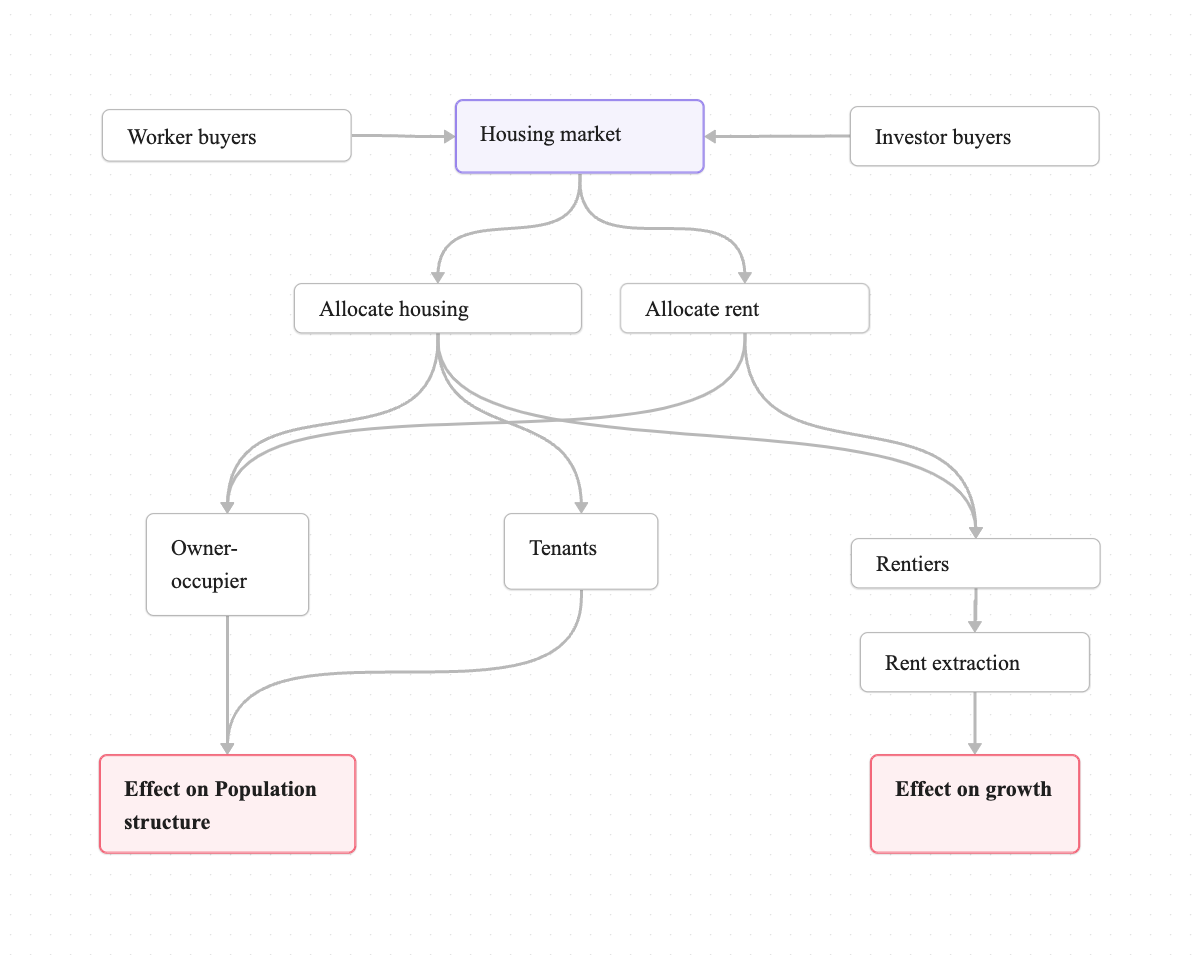
\includegraphics[scale=.90]{fig/flow_impacts.png}
    \label{Stylized model flow.}
\caption{Impacts.}
\end{adjustwidth}
\end{figure}


\begin{figure}
\vspace{-1cm}
\begin{adjustwidth}{-0.24\textwidth}{-0.24\textwidth}
    \centering
    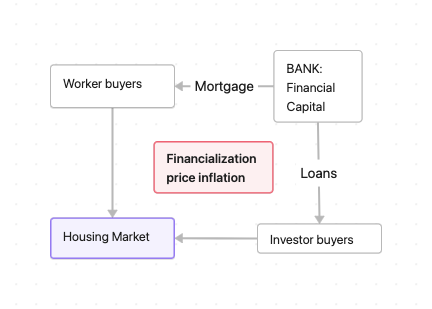
\includegraphics[scale=.90]{fig/flow_financialization.png}
    \label{Stylized model flow.}
\caption{Financialization.}
\end{adjustwidth}
\end{figure}

\begin{figure}
\vspace{-1cm}
\begin{adjustwidth}{-0.24\textwidth}{-0.24\textwidth}
    \centering
    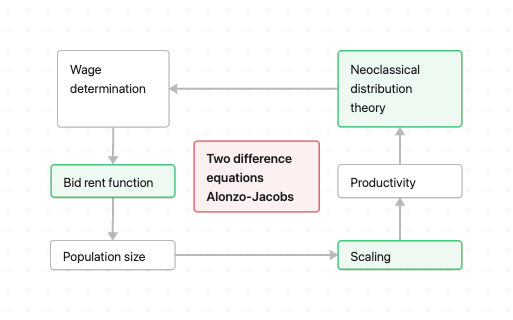
\includegraphics[scale=.90]{fig/flow_Alonzo-Jacobs_cycle.png}
    \label{Stylized model flow.}
\caption{The Alonzo-Jacobs cycle.}
\end{adjustwidth}
\end{figure}


 The idea of financialization of the housing market has been gaining a certain currency. This dissertation makes the case that it has implications for the success of cities. 

Financialization is ..

This dissertation focuses on implications for the success of cities..
develops a model to explore,
do do that has to develop ..

WHAT DO WE NEED FROM WHAT IS BELLOW? 


% SOMEWHERE IN THIS INTRODUCTION SAY THIS THESIS IS MODERN URBAN RENT THEORY. 

%Cities are the crucible of civilization, the hubs of innovation, the engines of wealth creation and centers of power, the magnets that attract creative individuals, and the stimulant for ideas, growth, and innovation." also dark side. "prime loci of crime, pollution, poverty, disease, and the consumption of energy and resources 214 [[West Scale]] ***E IF YOU WANT TO SAY THIS, MAKE SURE YOU CITE SOMETHING OR PROVIDE AT LEAST A MINIMAL CASE
 
%Missing- transfer of money vs put in a spatial framework.
%Most of the economic theory talks about where people go, and it doesn't talk about the value they create in the city and where that goes. That's finacialization, capturing those benefits is what capitalists are doing now.
% rent is being in the house/what they pay, the transfer of money, vs what cities are, and how that produces value..


% VERY SHORT PARAGRAPHS


COMMENT OUT HOUSING CRISIS STUFF AND OTHER IRRELEVANT STUFF!
Canada faces a housing crisis. The crisis now reaches far into the middle class, causing everything from declining home ownership rates to increasing poverty and displacement. 
%In the last few years, the need for affordable housing has come into focus as one of the most pressing issues facing Canadians. % ***E (ADD STRIKING STATISTIC - A NUMBER OR QUOTATION HERE.) 
% As more and more Canadians are finding 
%As more Canadians find housing unaffordable, the effects 
 % number of Canadians able to afford housing at all, leading to vacancies, poverty, and displaced workers. % (***E FILL THIS OUT A BIT - ADD SOME DETAILS HERE ABOUT THE EFFECTS OF THE CRISIS - THAT SET UP THE RESULTS OF THE THESIS)
% RATE OF INCREASE -VITAL SIGNS REPORT, CMHC
There has been extensive debate about the drivers of the crisis. ADD FACTS. Proposed explanations include supply shortages, stagnating incomes, and the financialization of housing ownership. 
% (Centering on two dominant stories, a story of supply and demand and one of rights.) %FIX and cite

There has been less work on the implications for productivity. 
In this thesis we focus on the financialization of housing ownership and its impact on urban productivity in an economy driven by urban agglomeration effects. 



%The source of the rents captured and the broader social and economic effects have not been fully captured. 
 %This provides insight into both population and wealth distribution in cities. 
%Integrating financial markets into the the spatial urban model allows us to examine the effect of financialization on cities, specificaly on their role in growth, distribution, and productivity. %the growth and wealth distribution of cities, and more specifically on their productivity effects. 
Our approach draws together insights from % economics and the study of cities. 
% Our model of the urban economy is based on work from %those developed in 
geography, planning and urban economics. 
The organizing principle in the spatial models of all three disciplines is an economic variable, land rent, which is for us the link to distribution, financialization and continuing productivity. %*** (another sentence on why this is great) --The space-less quality of the study of finance leaves out xyz GET PHRASING- CAN'T SEE- INTEGRATION OF SPACE NEGLECT GROWTH FACTOR. 

Rent is important is all these traditions, but has been neglected in modern theory. We argue that to formally understand the processes behind financialization and the housing crisis, what's needed is a modern urban theory of rent. This thesis is a contribution to the development of that theory. 

LINK
To capture urban productivity, we introduce %rely on 
agglomeration effects, relating existing spatial and growth models to the scaling models from the study of complexity. A fundamental feature in recent empirical work on scaling laws is % demonstrated in the recent literature on scaling laws: 
the persistent relationship between population and productivity. The productivity of cities increases superlinearly with population. Cities are the locus of a positive feedback loop with rising populations raising productivity, and rising productivity attracting more people and resource.




% Thus The productivity implications of the housing crisis are the focus of this thesis.

%(***E DEFINE TO SET UP THE DISTRIBUTIVE FEATURES OF ECONOMY). 
 % ***E ADD: the effects of housing affordability are pervasive / complex /run through the whole system / go far behind the obvious /direct effects / extend in non-obvious ways through the economy/whole system. What is at stake at a broader level is. 
% Yet, the economics is clear that what's at stake is the productivity of cities, the distributive features of the economy and the impact of the middle class % THIS IS A RESULT NOT AN INPUT. WHAT GOES HERE? ***E MAYBE ADD A CLARFIYING CONCLUDING SENTENCE HERE.... TO SAY SOMETHING LIKE THE EFFECTS OF HOUSING PRICES ARE NOT LIMITED TO 

% SAVE THIS ?? The greatest price increases have been in cities, where where people live and work, where  production is concentrated and where income is distributed. With humans becoming an increasingly an urban species, cities are a primary driver of technological development and increasing wealth. 

% (TIE BACK TO HOUSING CRISIS - EG. The affordability 
% \textbf{HOW WE ADD IT BACK IN}
%This thesis presents a spatial model of the city that incorporates distributional issues and financialization and allows us to examine the productivity implications of the housing crisis. The model that incorporates the scaling of productivity in cities within a standard urban model. 


%\textbf{WHY IT'S BEEN MISSING} EXPLAIN BETTER HERE WHY SPACE HAS BEEN LEFT OUT, AND WHY THAT LET'S US NEGLECTS SPATIAL RENTS AND MISS THE RELATION BETWEEN SPACE AND PRODUCTIVITY.
% We see urbanization and continuing and financialization accelerating. Financialization is driven by capital seeking profits, but what is the source of the rents they capture? The answer is in conventional urban theory, which allows us to identify the spatial distribution of those rents and traditional rent theory, which allows us to understand the social relations of those, those rents, the classical economists spend a great deal of time on that question. And we're very clear about it.
%We're talking about what is the puzzle? This is the teaser for this thesis and this thesis offers an answer to and I've just started to suggest that the teaser is given that 

% fig
% ***E I THINK THE PARAGRAPH ABOVE IS SAYING:  
% While financialization is usually understood as capital seeking prxfit, the source of the rents captured and the broader social and economic effects have not been fully captured.  XXXZ The current models for understanding financialization and it's effects don't predict the actual trends we are see. {\color{red} We argue this is because they miss the importance of space FIX.} 

%COMPELLING DESCRIPTION OF WHAT'S MISSING IN THE LITERATURE
%these share space, formalization in finance is spaceless

The housing crisis raises the question of whether Canadian cities can continue to attract people and accumulate wealth for its residents and industries, and whether they can sustain their growth.
% Our focus is land rents, %but in the context of an urban economy. 

Integrating classical and neoclassical economic approaches with traditional urban theory,  allows us to identify 
 we can build a more comprehensive model of financialization and its effects. This makes it possible to trace the spatial distribution of the rents.

This thesis  is thus a contribution to developing a modern theory of urban rents.

LINK/MOVE?
While financialization is usually understood as capital seeking profit, in the urban context it is a fundamentally spatial phenomenon. %also a spatial  phenomenon. 
Its goal is the capture of spatial rents, which, we will show, has implications for both the productivity and the class structure of the city. These aspects of finacialization in the urban system have been neglected in the literature. Standard models of the financial operations are spaceless.\footnote{In describing any theory we need to identify the kinds of objects that are theorized. Financial analysis theorizes  assets, debts, flows of revenue and costs, and the rates of change or exchange of these quantities over time. These are inherently spaceless because they are accounting entities, completely independent of location. It matters where a worker or a farm is. It does not matter where and dollar or a rouble is.} 
Our solution is to explicitly link the largely spaceless analysis of investment decisions to spatial rents in an urban system. 

%The effects of financialization on cities and economies has not been fully accounted for because the tools of the different, relevant disciplines have not been adequately integrated. The current approaches to describing the financialization of housing and its effects predict / explain /account for the housing crisis and effects on home ownership and access to housing, but our work shows that there are broader effects that have not been accounted for / predicted. 


% This fuller picture is made possible by bringing together classical rent theory, neo-classical XX and urban theory to create/and using/along with a agent-based model that allows us to .... (What the modelling technique enables) 

% \textbf{WHICH GIVES US THESE CONTRIBUTIONS}
% \section{Contributions}
%PROBABLY INTEGRATE WITH THE ABOVE, MAYBE MAP/HIGHLIGHT CONTRIBUTIONS IN A FIGURE/TABLE

%This work is important for understanding the current policy context. 
The analysis makes clear that in addition to the recognized distributional consequences, the housing crisis has productivity impacts that should be considered in developing urban and housing policy. Particularly, it centers concern with implication for urban development of growing rent extraction by the financial sector. 

\section{Position in the literature}
How does this fit in the larger literature?

The focus of this thesis is a topic that falls in the overlap between three academic  disciplines, Economics, Urban Geography, and Planning. % ***E mAYBE SUMMARIZE THE FOCUS OF EACH? While Economics traditionally focuses on... Urban Geography looks at ..... and Planning is the study of....
The central and shared concern in this area is with geographic space. % ***E DO YOU MEAN GEOGRAPHIC SPACE AND PEOPLE SOMEHOW? i FEEL LIKE YOU DON'T MEAN THIS? MAYBE MORE LIKE: The central shared concern between the three discipline it the role of geographic space in shaping WHAT? social and economic systems? human systems? society??


% \begin{figure}
% \begin{tikzpicture}{scale=.5}
% % find color cotrol for ball. Tind way to stop line short of node
% \coordinate (planning) at (-5,1);%PREFACE
% \coordinate (economics) at (5,.75);%
%  \coordinate (geography) at (-.5,-2); %history
% \coordinate (finance) at (0,5); %

% \draw [line width=2mm, black!15, ] (planning)--(economics);
% \draw [line width=2mm, black!20, ] (geography)--(economics);
% \draw [line width=2mm, black!20, ] (geography)--(planning);

% %\draw [line width=2mm, black!25, ] (geography)--(finance);
% %\draw [line width=2mm, black!20, ] (planning)--(finance);
% %\draw [line width=2mm, black!20, ] (finance)--(economics);

% \node [circle,shading=ball, minimum width=2.1   cm, white, align=center] (ball) at (planning) {Planning};
% \node [circle,shading=ball, minimum width=2.2cm, white, align=center] (ball) at (economics) {Economics};
% \node [circle,shading=ball, minimum width=3cm, white, align=center] (ball) at (geography)[text width=2cm] {\large Urban\\ Geography};

% %\node [circle, shading=ball, minimum width=2.4cm, white, align=center] (ball) at (finance)[text width=2cm] {Finance};

% \node at (-.3,-.1) [red] {\Large \textbf{Space}};
% \end{tikzpicture}
% \caption{The common concern of three fields topic }
%     \label{fig-three-fields}
% \end{figure}


A simple economic insight -- that locational value gives rise to land rents -- provides an organizing principle for % CUT the three disciplines where they overlap. 
% ***E REPLACE WITH: 
drawing the overlapping concerns of the three disciplines into a single coherent approach.

Locational value explains the spatial distribution of human activities because EXPLAIN. The distribution of locational rents or DEFINE... goes some distance to explaining core social issues like class structure, inequality, political political power and the dynamics of economic development.  ADD SUMMARIZING SENTENCE

%***E ADD:This thesis describes a model that draws together LIST HERE. 
To frame this approach to understanding current changes in our urban system we will now examine the development of the relevant theoretical tools, beginning with classical rent theory. % ***E OR list all??? ie. From Classical Rent to Neo-Classical Marginalist theory to XYZ urban theory and ...... etc. SET UP THE WHOLE SECTION.

The work is based on the concept of Classical Rent
Rent theory has a long history in economics, going back to thinkers such as Richard Cantillon (1680s-1734), François Quesnay (1694–1774), the marquis de Mirabeau (1715–1789) and Anne-Robert-Jacques Turgot (name physiocrat) and Adam Smith (1723-1790) and received its classic statement in Ricardo (1772-1823). %E ADD: The concept of rent illustrates WHAT in relation ot distribution, allows what kinds fo insights, which sets up this work.  We use the concept of rent to frame our consideration of how wealth is distributed in society by looking at WHAT?? how surplus is distributed? how locational value and location OR WHAT?? affects surplus distribution?? I dont know but please summarize how rent is used in this thesis. 

Nearly contemporaneous thinker, Johann Heinrich  von Th\"unen (1783-1850) developed a planning model to guide the location of economic activities for an urban-agricultural society.  A version of that model  was reinvented in urban geography by XXX. Alonzo\footnote{We use a version of the well-established model of Alonso (1964), Muth (1969) and Mills (1967), and formalised by Wheaton (1974),} % ***E NEED MORE DETAIL HERE ABOUT ALONZO"S MODEL, 

We link the Alonzo model with more recent work on growth theory starting with Robert Solo's XXX and with the endogenous growth models of Lucas () and draw on Jane Jacobs's insight that endogenous urban growth  is. now driving economic development. Jacobs's insight is empirically supported by recent work in the complexity literature on urban scaling by XXXX ()



\begin{figure}
    \centering
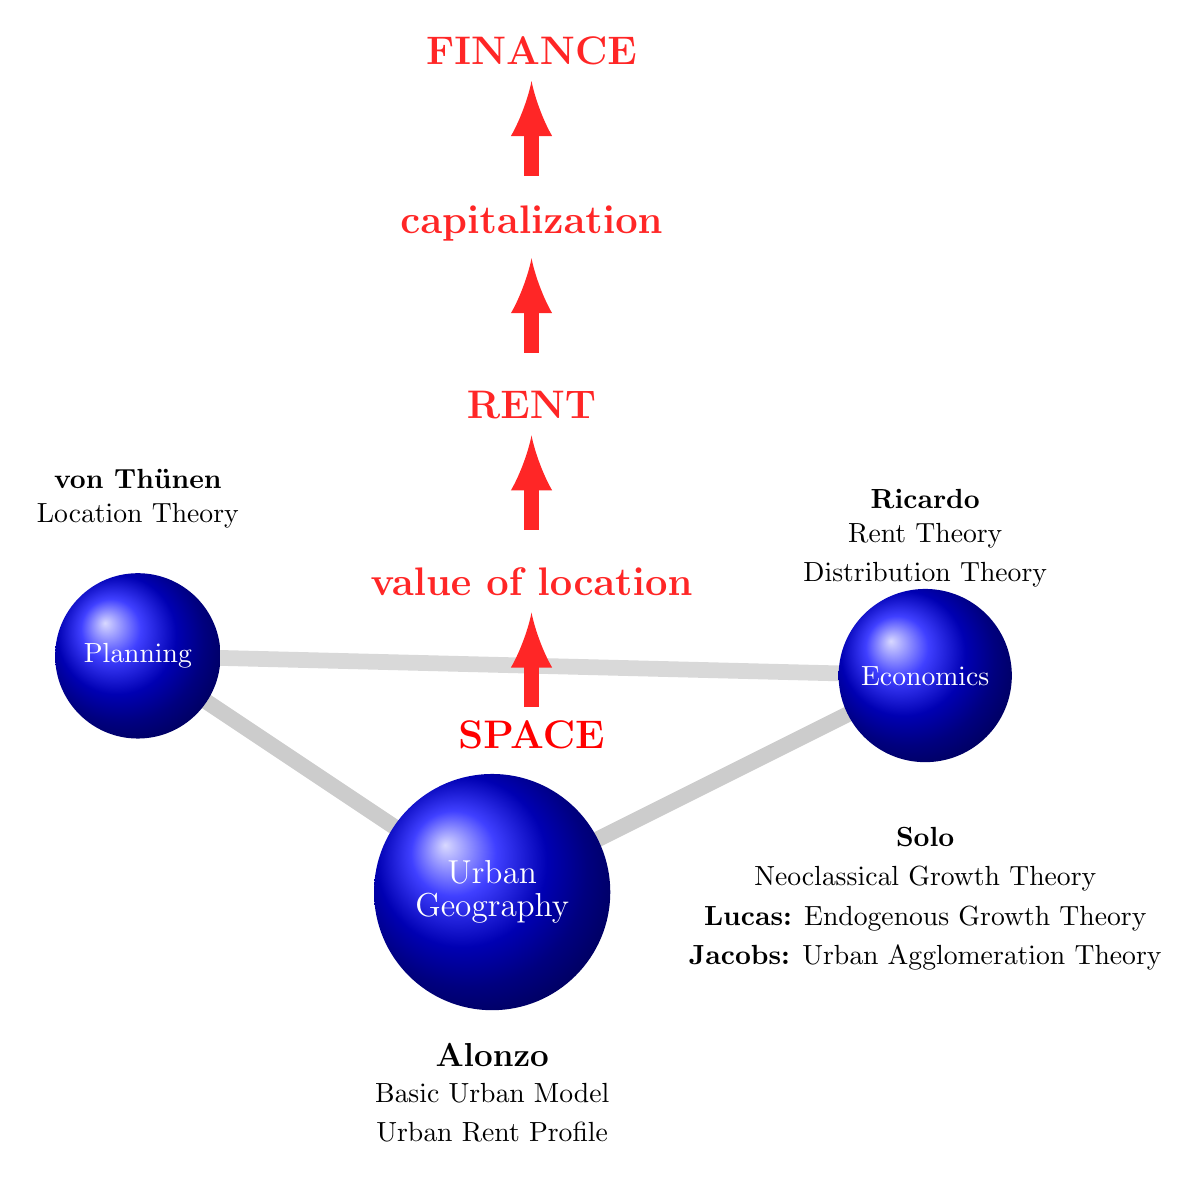
\begin{tikzpicture}{scale=.5}
% find color cotrol for ball. Tind way to stop line short of node
\coordinate (planning) at (-5,1);%PREFACE
\coordinate (economics) at (5,.75);%
 \coordinate (geography) at (-.5,-2); %history
\coordinate (finance) at (0,5); %

\draw [line width=2mm, black!15, ] (planning)--(economics);
\draw [line width=2mm, black!20, ] (geography)--(economics);
\draw [line width=2mm, black!20, ] (geography)--(planning);

%\draw [line width=2mm, black!25, ] (geography)--(finance);
%\draw [line width=2mm, black!20, ] (planning)--(finance);
%\draw [line width=2mm, black!20, ] (finance)--(economics);

\node [circle,shading=ball, minimum width=2.1   cm, white, align=center] (ball) at (planning) {Planning};
\node [circle,shading=ball, minimum width=2.2cm, white, align=center] (ball) at (economics) {Economics};
\node [circle,shading=ball, minimum width=3cm, white, align=center] (ball) at (geography)[text width=2cm] {\large Urban\\ Geography};

%\node [circle, shading=ball, minimum width=2.4cm, white, align=center] (ball) at (finance)[text width=2cm] {Finance};

%\node at (-.3,-.1) [red] {\Large \textbf{RENT}};

% new stuff
\node at (planning) [above=2cm] {\textbf{von Th\"unen}};
\node at (planning) [above=1.5cm] {Location Theory};

\node at (economics) [above=2cm] {\textbf{Ricardo}};
\node at (economics) [above=1.5cm] {Rent Theory};
\node at (economics) [above=1.0cm] {Distribution Theory};

\node at (economics) [below=1.8cm] {\textbf{Solo}};
\node at (economics) [below=2.3cm] {Neoclassical Growth Theory};
\node at (economics) [below=2.8cm] {\textbf{Lucas:} Endogenous Growth Theory};
\node at (economics) [below=3.3cm] {\textbf{Jacobs:} Urban Agglomeration Theory};


\node at (geography) [below=1.8cm] {\textbf{\large Alonzo}};
\node at (geography) [below=2.3cm] {Basic Urban Model};
\node at (geography) [below=2.8cm] {Urban Rent Profile};

%\node [circle, shading=ball, minimum width=2.4cm, white, align=center] (ball) at (finance)[text width=2cm] {Finance};
\draw [line width=2mm, red!85, -latex ] (0, 7.1)--++(0,1.2)node[above=-.1] {\Large \textbf{FINANCE}};
\draw [line width=2mm, red!85, -latex ] (0, 4.85)--++(0,1.2)node[above=-.1] {\Large \textbf{capitalization}};
\draw [line width=2mm, red!85, -latex ] (0, 2.6)--++(0,1.2)node[above=-.1] {\Large \textbf{RENT}};
\draw [line width=2mm, red!85, -latex ] (0, .35)--++(0,1.2)node[above=-.1] {\Large \textbf{value of location}};
\node at (0,0) [red] {\Large \textbf{SPACE}};


\end{tikzpicture}

    \caption{space and value ***TODO FLIP ECON AND PLANNING TO FOLLOW ORDER OF CHAPTERS}
    \label{fig-space-value}
\end{figure}

Land rent was historically the basis of the wealth and political power of  the land-owning class in the era of the classical economists. % ***E NEED MORE HERE


We further link the model of urban rents to emerging concerns about the financialization of the housing market. The key insight we offer is that the financialization  of the housing sector is a  form of rent-seeking that must have detrimental effects on urban development and on the well-being of urban residents.


% ***E NEED TO POSITION THIS WORK IN RELATION TO THE MARGINALIST ACCOUNT IN THIS SECTION BECAUSE IT IS ONE OF THE FEW THINGS YOU HAVE INTRODUCES. tHE URBAN MODELS YOU DESCRIBE HERE SHOULD BE FRAMED BY WHAT YOU ADD IN BACKGROUND ABOUT PLANNING/URBAN MODELS (AS PER MY SUGGESTION IN THAT SECTION) 
% ***E YOU ALSO NEED TO ADD A SUMMARIZING PARAGRAPH WHICH I CAN HELP WRITE WHEN THIS SECTION IS MORE FILLED OUT. MAYBE THIS:
% ***E ADD: By bringing these approaches into a coherent approach, we can better account for  WHAT... EXPLAIN THAT alone they don't give as complete a picture. This thesis show that certain things become clear when they are brought together that provide an better account of the current situation. Older economics models do not predict certain things that are currently happening. This is because they are based on out of date modes of production, fail to account for the importance of location value and the modelling tools available when they were developed required some simplification.   Updating the models for the changing times, using more complex modelling systems and incorporating space with the economic models allow us to create models and narratives that provide a more effective understanding of the situation as it stands today. 





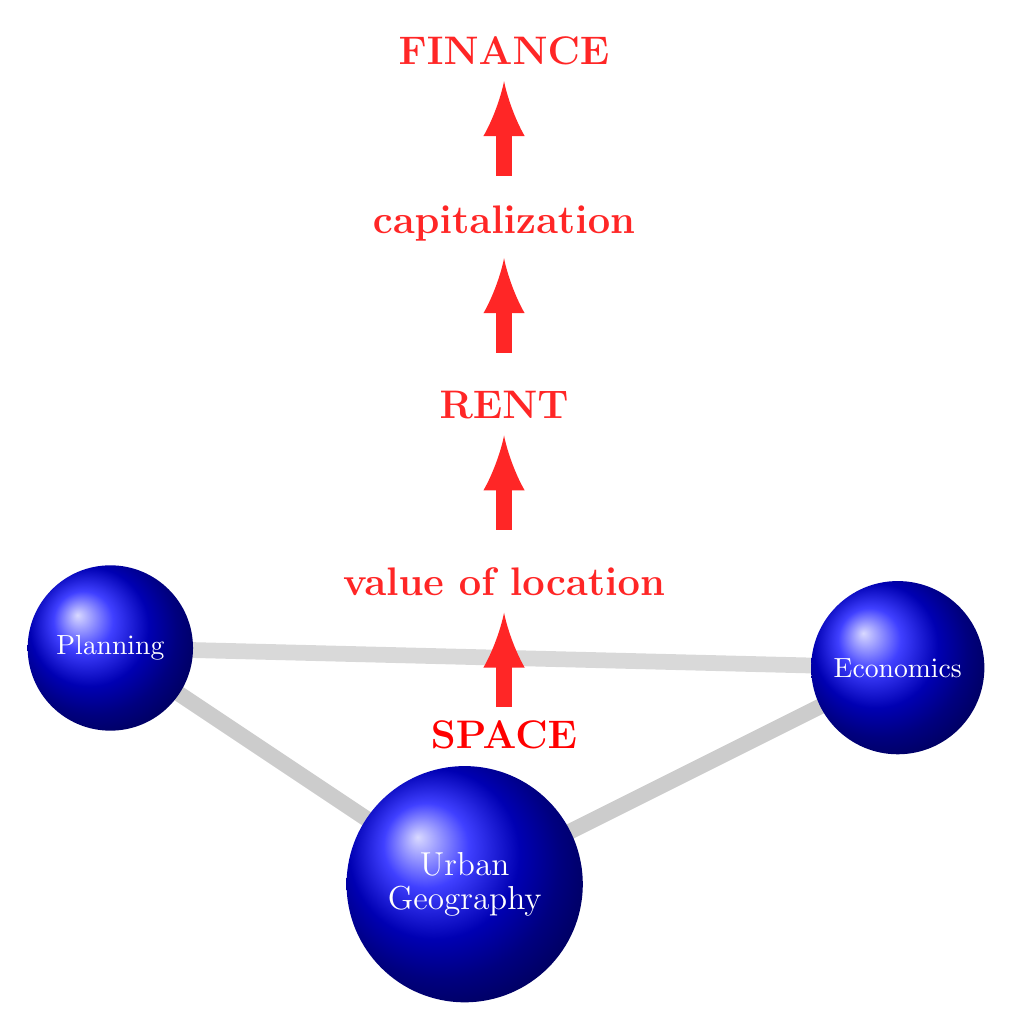
\begin{tikzpicture}{scale=.5}
% find color cotrol for ball. Tind way to stop line short of node
\coordinate (planning) at (-5,1);%PREFACE
\coordinate (economics) at (5,.75);%
 \coordinate (geography) at (-.5,-2); %history
\coordinate (finance) at (0,5); %

\draw [line width=2mm, black!15, ] (planning)--(economics);
\draw [line width=2mm, black!20, ] (geography)--(economics);
\draw [line width=2mm, black!20, ] (geography)--(planning);

%\draw [line width=2mm, black!25, ] (geography)--(finance);
%\draw [line width=2mm, black!20, ] (planning)--(finance);
%\draw [line width=2mm, black!20, ] (finance)--(economics);

\node [circle,shading=ball, minimum width=2.1   cm, white, align=center] (ball) at (planning) {Planning};
\node [circle,shading=ball, minimum width=2.2cm, white, align=center] (ball) at (economics) {Economics};
\node [circle,shading=ball, minimum width=3cm, white, align=center] (ball) at (geography)[text width=2cm] {\large Urban\\ Geography};

%\node [circle, shading=ball, minimum width=2.4cm, white, align=center] (ball) at (finance)[text width=2cm] {Finance};
\draw [line width=2mm, red!85, -latex ] (0, 7)--++(0,1.2)node[above=-.1] {\Large \textbf{FINANCE}};
\draw [line width=2mm, red!85, -latex ] (0, 4.75)--++(0,1.2)node[above=-.1] {\Large \textbf{capitalization}};
\draw [line width=2mm, red!85, -latex ] (0, 2.5)--++(0,1.2)node[above=-.1] {\Large \textbf{RENT}};
\draw [line width=2mm, red!85, -latex ] (0, .25)--++(0,1.2)node[above=-.1] {\Large \textbf{value of location}};
\node at (0,-.1) [red] {\Large \textbf{SPACE}};
\end{tikzpicture}



% \vspace {2cm}
% Figure 4 with finance

% \begin{tikzpicture}{scale=.5}
% % find color cotrol for ball. Tind way to stop line short of node
% \coordinate (planning) at (-5,1);%PREFACE
% \coordinate (economics) at (5,.75);%
%  \coordinate (geography) at (-.5,-2); %history
% \coordinate (finance) at (0,5); %

% \draw [line width=2mm, black!15, ] (planning)--(economics);
% \draw [line width=2mm, black!20, ] (geography)--(economics);
% \draw [line width=2mm, black!20, ] (geography)--(planning);

% \node at (-.3,2) [red] {\huge \textbf{RENT}};

% \draw [line width=3mm,  black!50,opacity=.5 ] (geography)--(finance);
% \draw [line width=2mm, black!20, ] (planning)--(finance);
% \draw [line width=2mm, black!20, ] (finance)--(economics);

% \node [circle,shading=ball, minimum width=2.1   cm, white, align=center] (ball) at (planning) {Planning};
% \node [circle,shading=ball, minimum width=2.2cm, white, align=center] (ball) at (economics) {Economics};
% \node [circle,shading=ball, minimum width=3 . cm, white, align=center] (ball) at (geography)[text width=2cm] {\large Urban\\ Geography};

% \node [circle, shading=ball, minimum width=2.4cm, white, align=center] (ball) at (finance)[text width=2cm] {Finance};


% \end{tikzpicture}



\vspace {2cm}
Figure 4 with finance

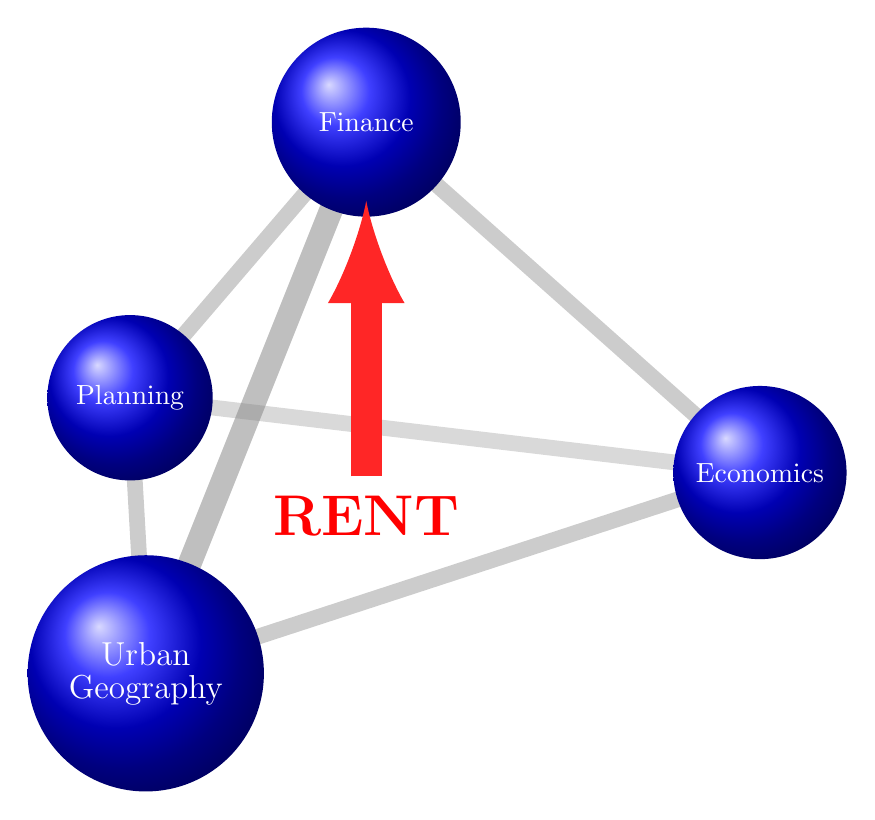
\begin{tikzpicture}{scale=.5}
% find color cotrol for ball. Tind way to stop line short of node
\coordinate (planning) at (-3,1.5);%PREFACE
\coordinate (economics) at (5,.55);%
 \coordinate (geography) at (-2.8,-2); %history
\coordinate (finance) at (0,5); %

\draw [line width=2mm, black!15, ] (planning)--(economics);
\draw [line width=2mm, black!20, ] (geography)--(economics);
\draw [line width=2mm, black!20, ] (geography)--(planning);

\node at (.0,0) [red] {\huge \textbf{RENT}};

\draw [line width=3mm,  black!50,opacity=.5 ] (geography)--(finance);
\draw [line width=2mm, black!20, ] (planning)--(finance);
\draw [line width=2mm, black!20, ] (finance)--(economics);

\node [circle,shading=ball, minimum width=2.1   cm, white, align=center] (ball) at (planning) {Planning};
\node [circle,shading=ball, minimum width=2.2cm, white, align=center] (ball) at (economics) {Economics};
\node [circle,shading=ball, minimum width=3cm, white, align=center] (ball) at (geography)[text width=2cm] {\large Urban\\ Geography};

\node [circle, shading=ball, minimum width=2.4cm, white, align=center] (ball) at (finance)[text width=2cm] {Finance};
\draw [line width=4mm, red!85, -latex ] (0, .5)--(0,4);
\end{tikzpicture}

\section{Contributions}
The main contributions, % methodological innovations
as we see it, are ROUGH LIST. TO SUMMARIZE AND SORT:

% \begin{enumerate}
%     \item we incorporate \gls{classical rent theory} into an agent-based urban model 
%     \item we allow the creation and distribution of rents to influence urban growth, productivity and  population structure. 
%     \item we incorporate current research on \gls{urban scaling} into the  core spatial urban model.   
%     \item we construct an   Urban \gls{ABM} that is consistent with \gls{neoclassical growth theory},
%     \item we integrate \gls{financial capital} into a standard spatial model of the urban system
%     \item we integrate financial capital into an population model of the urban system
%     \item we employ the ABM to examine how financial markets impact the urban land markets 
%     \item we test for \gls{hysteresis}  resulting from the business cycle  in the urban system 
%     \item we build a model that is easily extended to explore a wide range of issues
%     \item we provide a model that we believe can be used  to evaluate urban policies
% \end{enumerate}

Each of the items above requires us to  integrate models and concepts from different parts of the literature. 

ADD TO EACH: THIS MEANS, THIS MATTERS BECAUSE, THEN FOLLOW WITH TO DO IT, WE NEED TO.

% CONSIDER MENTIONING WHAT ORDER THIS IS IN  % It's a kind of logical order, almost in the order of development: (types, order implemented, order theory is developed, order of importance?)

IS THERE A PICTURE THAT COULD ILLUSTRATE THE CONTRIBUTIONS?

\begin{enumerate}
    \item incorporating \gls{classical rent theory} into an agent-based urban model 

This requires a how Ricardian rent theory - a theory of distribution based on an agricultural economy - applies in an economy driven by human capital agglomeration effects within the urban system. 

    \item allowing the creation and distribution of rents to influence urban growth, productivity and  population structure. 
    
This requires us to articulate the links between the wealth production of cities and  urban systems evolve 

    \item incorporating current research on \gls{urban scaling} into the  core spatial urban model.  

We show how understanding how complex systems scale provides an elegant way to model a an urban system with production

    \item constructing an urban \gls{agent-based model} that is consistent with {neoclassical growth theory},

% Although many  who employ ABMs to analyse urban systems are deeply skeptical of neoclassical assumptions
We demonstrate in this context how %easily and productively 
the neoclassical framework can be implemented in the agent-based framework, and make a case for it's usefulness in linking urban rents and productivity, linking traditions that have been seperate. 

In general, there is relatively little work rigorously linking analytic and agent based models, so the results can be understood formally, in relation. % incorporated into prior traditions and

    \item integrating \gls{financial capital} into a standard spatial model of the urban system

% We are not aware of any urban simulation models that
We introduce capital within this framework in a novel way. %as we do to examine the outcomes that concern us.
    
    \item integrating financial capital into an \gls{overlapping generations} population model of the urban system

Financial assets are central to most overlapping generations models. Our innovation is to articulate the movement of financial capital though the urban land market. 

SOMETHING LIKE Adding space to finance which has been spaceless.
    
    \item using an ABM to examine how financial markets impact  urban \glspl{land market}.

We began with with the fact that there is growing policy concern about the ``Financialization of  Housing''. We have produced a formal simulation model that illustrates the process. 

    \item testing for \gls{hysteresis} resulting from the business cycle   in the urban system, exploring the \gls{resilience} implication's of the core spatial economic model

There are two types of resilience questions when any system is shocked, does it return to an https://www.overleaf.com/project/606a6b286ae1c9f203fadab5equilibrium state - the stability question - and does it return to the same kind of equilibrium - the hysteresis question. We focus on the latter question.  

    \item building a model that is easily extended to explore a wide range of issues

The model combines clear and explicit theoretical assumptions with careful and transparent implementation of the logic in flexible Python code.

    \item providing a model that we believe can be used  to evaluate urban policies

To be useful in policy discussions, a model must correctly simulate the relevant system features and be able to incorporate a variety of policy interventions. We have taken care to allow for  both theoretical and policy- relevant extensions in the way the simulation model is coded. 
\end{enumerate}

(** ``The notion that your labour force is on average more productive when there are more people around is pretty dramatic and it's very much not part of the basic model that we use. Our starting point is that's the fundamental feature of cities, and what does that do with financial capital and what does that do to distribution and that's not been explored. PUT THIS IDEA HERE?)

\section{Document overview}
This thesis develops a conceptual framework for a model of the housing market and then describes the model and the implications of the analysis of the model. %insights it produces. 
There are three parts in the dissertation. 

MAYBE LINK ORDER TO POSITION IN THE LIT/CONTRIBTUIONS AGAIN % 3 PARTS TO THE MODEL, DEVELOPMENT FOLLOWS THE TRAJECTORY OF THIS. 

Part \ref{part-background} gives the background and introduces the theoretical framework for the analysis,  linking classical rent theory, neoclassical production theory, neoclassical growth theory, the scaling literature, and urban spatial models. 

\begin{enumerate}
    \item Chapter \ref{chapter-background} sketches how this thesis relates to four major fields: classical rent theory, neoclassical production theory and growth theory, the scaling literature, and urban spatial models. %..., and the role of space as a unifying factor across three of the fields. % WITH FINANCE IS SPACELESS.
    % *** ADD BACK? This work draws together sub-literatures including rent theory, production functions, the standard urban model, growth theory, urban growth theories, financialization, and the theory of distribution, so the chapters review those areas. % *** link the areas to the chapters better?  %theory for our analysis, 
    \item Chapter \ref{chapter-rent} reviews the literature on rent and develop an approach suited to the analysis for this work.
    \item Chapter \ref{chapter-growth} introduces growth theory, showing how our model is directly connected with this broad collection of linked theories. %, we use the Cobb-Douglas function, which is used across this entire range of literature - frame the relation of a tradition in context of  % After we develop the mathematical description of the relationship among these will discuss  in more detail, rent theory and our contribution, scaling laws, ......  and other issues in the literature that draw on parts of this model and % ???  apply to the specific situation we're in why rent theory is related to discussions of exploitation why it might lead the inefficiencies, whether or not this links with other important models in the literature.
    \item Chapter \ref{chapter-space} develops the urban model of space drawing on the basic Alonzo model.
    \item Finally Chapter \ref{chapter-financialization} provides a description of finacialization, and explores the potential consequences of fiancialization in the housing market.  % showing it is a form of rent-seeking in the housing market and ?? 
\end{enumerate}
 
Part \ref{part-model} develops the model and results.
\begin{enumerate}
    \item Chapter \ref{chapter-methodology} introduces the methodology. % In addition to the core contribution linking housing and productivity, there are three methodological lines of contribution, and there are policy implications SUMMARIZE METHODOLOGICAL CONTRIBUTIONS %(rent is key to financialization, however the main urban models don't observe the distribution of rents)
    \item Chapter \ref{chapter-model} describes an illustrative agent-based model of the urban system. 
    This model has three  parts, first a production function, modelling how urban regions generate wealth, and second a model of an urban housing market, and finally, a financial sector that can participate in the market. 
% Alternative phrasing 
%We integrate a labour market into a spatial urban model, set up to explore rent, and implications for the distribution of wealth.

\textbf{The model has a Solow-Swan style production model with agglomeration effects using a \gls{Cobb-Douglas} production function that incorporates Jacobs-style labour-augmenting agglomeration economies %(Beaudry and Schiauerova 2009, Panne 2004, J. Jacobs 1969), 
in the way neoclassical growth theory incorporates labour-augmenting technical change.}
It integrates the production function with an Alonso-style urban model of a city economy (Alonso 1964). 

We take a step beyond integrating labour markets in a city, to studying the distributional effects: who gets the surplus, what does that mean for the class structure, and ultimately the productivity of cities. 

This chapter introduce the urban spatial model and labour supply, models the production function with urban scaling of agglomeration effects with density, then introduces a model of financial investment/speculation into a spatially explicit land market model, then calculates profit, considers who gets the profit, and draws conclusions. 
 %calculate the urban surplus, and consider who gets it. 
 
MOVE TO LIT REVIEW/CONTRIBUTION?
%: The work draws on the Alfonso/Von Thünen model of the concentric city and Dawn Parker and Filatova's work in agent-based modelling of housing markets (see http://jasss.soc.surrey.ac.uk/12/1/3.html 2009).% We begin with a simple model of a circular city with urban agglomeration effects. In subsequent sections we will use an agent-based model to relax assumptions to look at how the interaction between the production of social wealth in cities interacts with housing and the extraction of rent to drive patterns for individuals over space and time.
Most of the analysis of urban systems has employed analytical models with roots that go back to von Thunen () and more recently Alonzo. These models are extremely useful, but necessarily abstract from the concrete  and variable individual behaviour and  the details  of dynamics that make real cities path-dependent. XXX (Dawn) have shown that agent-based models can reproduce the features of the analytical models, at least in simple cases. TODO maybe divide chapter on theoretical core, followed by chapter on impelementation (general for basic and resilience experiments).
    \item TODO experiment 1 - setup, parameter values,  analysis, and results
    \item Chapter \ref{chapter-resilience} develops a resilience analysis of the effects of a driven version of the model, introducing the pump effects.  

Experiment 2 - setup, parameter values,  analysis, and results (TODO maybe introduce resilience ideas earlier so they are part of the mainline development, adding a resilicen theory to part  \ref{chapter-background} after chapter \ref{chapter-financialization}.
\end{enumerate}

 Finally Part \ref{part-system} puts the analysis %model %and theory 
in the context of a larger system, using methods of systems analysis and design, to discusses potential interventions and policy implications.
\begin{enumerate}
    \item Chapter \ref{chapter-interventions} considers the system, examines the potential for a range of interventions, and identifies policy implications. % with a diagram relating interventions.
    \item TODO chapters .. may analyze particular interventions/cases in more detail: e.g. shared ownership models e.g. acquisition/land trusts, developer models, tax/zoning, and funds/financing.
\end{enumerate}

% After we develop the mathematical description of the relationship among these will discuss in more detail, various relevant applications, and issues in the literature that draw on parts of this model and apply to the specific situation we're in why rent theory is related to discussions of exploitation why it might lead the inefficiencies, whether or not this links with other important models in the literature.

% Because we draw on a wide range of methods and literatures, we discuss the relevant literature and  methodologies in the chapters where they apply 